\chapter{Související práce a pojmy}
\label{chap:teoreticka_cast}

V této části popisujeme komplikovanější teoretické koncepy používané v práci a
práce s podobným zaměřením.


\section{Zeměpisné souřadnice a sférická vzdálenost}
\label{sect:zem_souradnice}

\emph{Zeměpisné souřadnice}  slouží k určování polohy na povrchu Země. Nejčastěji 
jsou udávány jako trojice \emph{zeměpisná šířka} (anglicky latitude), 
\emph{zeměpisná délka} (anglicky longitude) a nadmořská výška. V naší práci
využíváme první dva údaje (tedy zeměpisnou šířku a délku).
K určení vzdáleností mezi body na sféře u nichž známe jejich zeměpisné 
souřadnice se používá takzvaná \emph{haversinová formule}. 
Podrobněji popisuje problematiku \citet{chang2008introduction}.


\section{Genetický algoritmus}
\label{section:genetic_alg}
\emph{Genetický algoritmus} (GA) je heuristický algoritmus, jehož cílem je pomocí
aplikace principů evoluční biologie nalézt řešení problémů, pro něž neexistuje
použitelný exaktní algoritmus. Existuje mnoho variant GA a popis všech by byl
vyčerpávající. Popíšeme tedy pouze variantu používanou v této práci. Podrobnější
popis genetického algoritmu popisuje \citet{mitchell1998introduction}.

Princip řešení problému je založen na evoluci generací jedinců, kde každý z nich
reprezentuje jedno řešení daného problému. První generace je typicky 
inicializována náhodně. Každý jedinec je ohodnocen \emph{fitness funkcí}, která 
vyjadřuje kvalitu řešení. Na základě této funkce jsou následně stochasticky vybráni (tzv. selekce) 
jedinci (rodiče), jež jsou pomocí tzv. \emph{genetických operátorů}, mezi něž 
patří \emph{křížení} a  \emph{mutace},
modifikováni v nové jedince následující generace. Tento postup je iterativně opakován s 
očekáváním zlepšující se kvality řešení a je ukončen po dosažení zvolené 
ukončovací podmínky (typicky dostatečná kvalita řešení, dosažení maximálního
počtu iterací, malá změna fitness mezi generacemi apod.).

Individua (rodiče) pro křížení vybíráme tzv. \emph{turnajovou selekcí}, 
v níž nejprve náhodně zvolíme 2 jedince a z 
nich vybereme se zvolenou vyšší pravděpodobností jedince s lepší fitness. 
Takto dostaneme individua, na nichž budeme následně aplikovat 
genetické operátory. Část nové populace vznikne zkopírováním zvoleného počtu 
jedinců s nejlepším ohodnocením z aktuální generace do nové generace. Takto je 
zajištěno, že v nové generaci bude vždy zastoupen jedinec s aktuálně nejlepším
ohodnocením. Selekce vybírá tolik jedinců, aby nová generace obsahovala stejný
počet jedinců, jako to předešlá.

Po selekci rodičů následuje křížení, jehož výsledkem jsou dva noví jedinci
vzniklí kombinací obou rodičů. V naší práci volíme \emph{jednobodové křížení},
kde je zvolen bod v jedinci, jenž určuje část jedince, která
je vyměněna mezi rodiči. Předpokladem jednobodového křížení je reprezentace
jedince posloupností parametrů (aby bylo možné zvolit bod v posloupnosti, od 
něhož je zbylá část vyměněna s částí druhého rodiče).

Na nových jedincích vzniklých křížením je následně aplikována mutace.
Zde jsou s malou pravděpodobností náhodně změněny jednotlivé
části jedince (tzv. geny). Cílem mutace je především zabránit vzniku 
jednotvárné populace.

\begin{algorithm}
\begin{algorithmic}
\Function{Genetický algoritmus}{}
    \State Náhodná inicializace populace.
    \While{ukončovací podmínka není splněna}
        \State Zvol jedince pro další generaci (selekce).
        \State Zkombinuj zvolené jedince (křížení).
        \State Náhodně pozměň nové jedince (mutace).
    \EndWhile

\EndFunction
\end{algorithmic}
\caption{Pseudokód genetického algoritmu.}
\label{alg:genetic_alg}
\end{algorithm}


\section{K-Means}
\label{sec:kmeans_alg}
Algoritmus \emph{k-means} je příkladem \emph{shlukovací metody}. 
Předpokládáme, že shlukované objekty lze chápat jako body v metrickém prostoru 
a počet shluků je pevně zvolen na začátku algoritmu (ozn. jako $k$). 
Každý shluk je reprezentován \emph{centroidem}.
Jedná se o bod v prostoru, jenž typicky reprezentuje střed daného shluku bodů.  
Pozice centroidů v první iteraci algoritmu jsou typicky voleny náhodně, nebo
pomocí vhodně zvolené heuristiky (jako ochrana před konvergencí k nesprávnému
lokálnímu optimu).
V průběhu algoritmu jsou objekty přiřazovány do shluku, jehož centroid
je nejblíže od objektu. Tento krok označujeme jako \emph{E-krok}. Po rozdělení 
objektů do shluků je aktualizována pozice centroidu daného shluku, 
tak aby ležel v těžišti shluku (typicky se jedná o průměrnou pozici všech 
objektů ve shluku). Tento krok se typicky označuje jako \emph{M-krok}. 
Po aktualizaci centroidů jsou body přiřazeny do nových shluků a postup výše
je iterativně opakován do doby, než se poloha centroidů ustálí.

V reálných aplikacích často nevíme, jaké $k$ zvolit. Tento problém se typicky 
řeší spuštěním algoritmu s různými hodnotami $k$ a na základě požadovaných
parametrů je následně zvolena nejlepší hodnota $k$. Podrobněji popisuje 
problematiku \citet{macqueen1967classification}.

\begin{algorithm}
\begin{algorithmic}
\Function{K-Means}{}
    \State Náhodná inicializace centroidů.
    \While{změna pozice centroidů}
        \State Roztřiď objekty do nejbližších shluků.
        \State Spočítej novou pozici centroidů.
    \EndWhile

\EndFunction
\end{algorithmic}
\caption{Pseudokód algoritmu K-Means.}
\label{alg:kmeans_alg}
\end{algorithm}


\begin{figure}
    \centering
    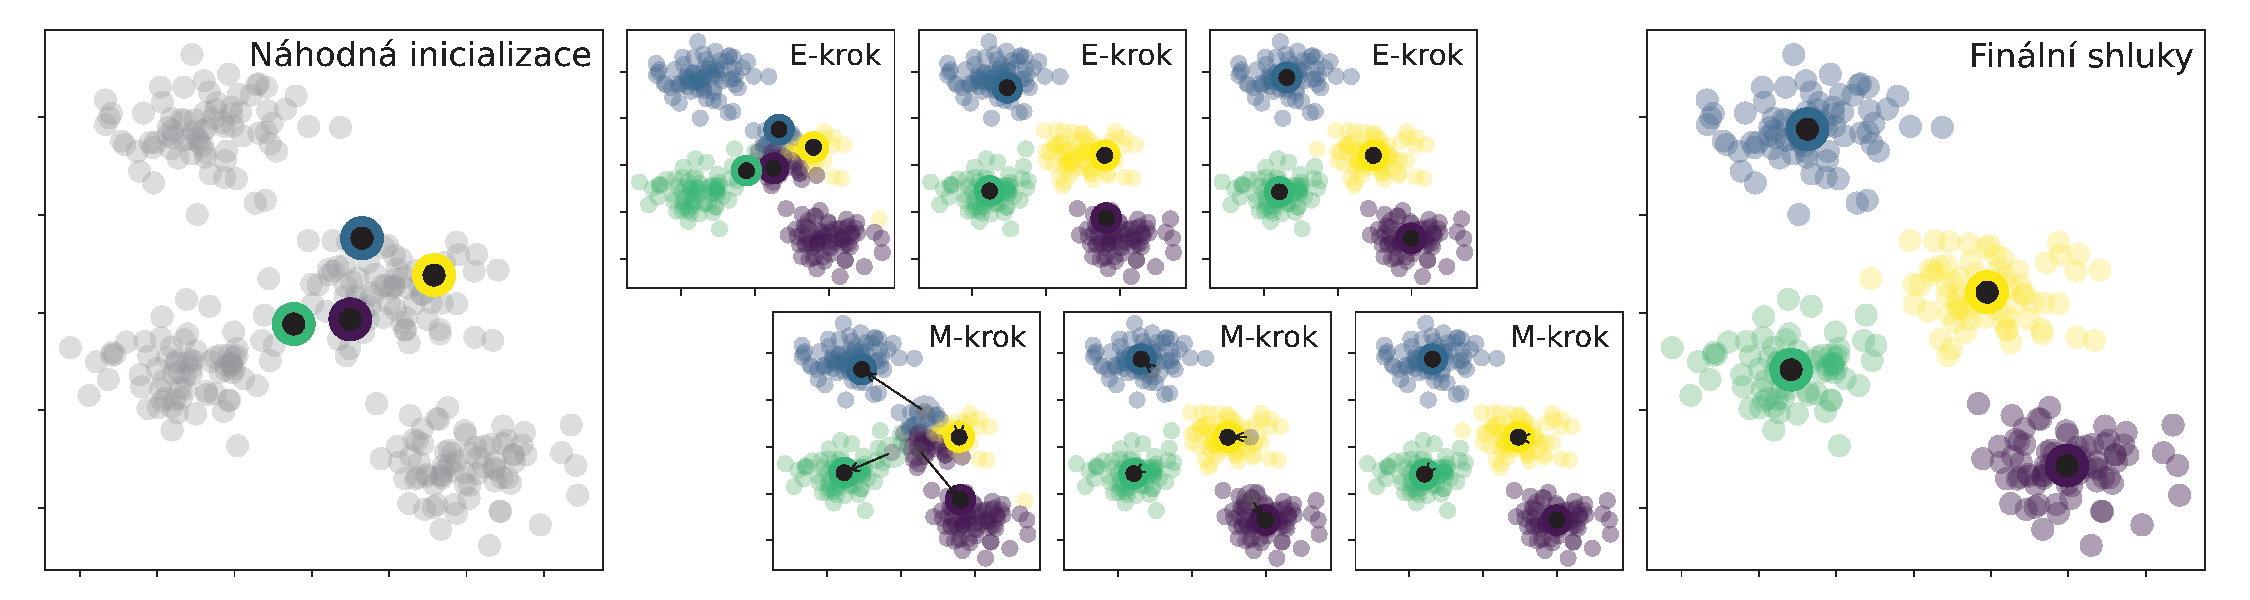
\includegraphics[width=1\linewidth]{img/pdfa-kmeans_example.pdf}
    \caption{Příklad průběhu algoritmu k-means. Černé kruhy značí centroidy, 
    barevné lemování slouží k jejich odlišení. Barva jednotlivých bodů
    značí náležení bodu do shluku centroidu s příslušnou barvou.}
    \label{fig:kmeans_example}
\end{figure}


\section{A-star}
\label{sec:a_star}
\emph{A-star} (A*) je algoritmus pro vyhledávání optimálních cest v kladně 
ohodnocených grafech. Jedná se o modifikaci Dijkstrova algoritmu s přidaným 
heuristickým prvkem.

Výpočet algoritmu je téměř totožný s Dijkstrovým algoritmem, od něhož se 
odlišuje ve výběru následujícího vrcholu pro otevření, který volí na základě
funkce $f(x) := g(x) + h(x)$. Funkce $g(x)$ zde označuje reálnou (nalezenou) 
vzdálenost od počátečního bodu do bodu $x$ (Dijkstrův algoritmus pracuje pouze 
s touto hodnotou). Funkce $h(x)$, pak značí heuristickou funkci odhadující 
vzdálenost vrcholu $x$ od požadovaného cílového vrcholu. Pokud je heuristická 
funkce vhodně zvolena, je možné znatelně omezit počet operací pro nalezení nejkratší
cesty mezi dvěma vrcholy v porovnání s Dijkstrovým algoritmem. 

Typicky je u heuristické funkce $h$ požadována tzv. \emph{přípustnost} 
(nenahodnocuje vzdálenost do cíle), či \emph{monotónost} 
(hodnota funkce $h$ roste po přechodu na další hranu), více
informací o tomto algoritmu popisuje \citet{russell2010artificial}.


\section{Související práce}
\label{sec:souvisejici_prace}

V této sekci si popíšeme několik souvisejících prací a stručně popíšeme 
jejich vlastnosti.


Simulátor SUMO\footnote{\url{https://www.eclipse.org/sumo/}} je velmi detailní
simulátor dopravy v rozsahu funkcionalit zdaleka přesahující naši implementaci.
V programu lze do jisté míry simulovat také elektromobily. Pro naše učely je
ale tento program velmi komplexní a práce s optimalizačními algoritmy
by tak byla neprakticky komplikovaná.

Simulátor City Flow\footnote{\url{https://cityflow.readthedocs.io/en/latest/index.html}}
se pyšní především výpočetní efektivitou\footnote{\url{https://cityflow.readthedocs.io/en/latest/introduction.html}}.
Bohužel nenabízí jednoduché uživatelské rozhraní pro rozšíření o metody
potřebné pro naši optimalizaci.

V práci \citet{kmeans_layout} je navržen simulátor dopravy pro následnou 
analýzu nově navrženého optimalizačního algoritmu rozmístění nabíjecích stanic
na území Japonska. Optimalizační algoritmus v práci se snaží minimalizovat 
počet vozidel, kterým se vybila baterie, pomocí posunů nabíjecích stanic směrem
k místům, kde se v minulosti vybila baterie vozidla. Návrh simulátoru naší práce
a optimalizační algoritmus s použití metody k-means jsou inspirovány zmíněnou
prací.

V práci \citet{niccolai2021optimization} je zkoumáno několik variant evolučních
algoritmů pro optimalizaci rozmístění nabíjecích stanic elektrických vozidel
ve městě Milán. V práci byl porovnáván také hladový přístup rozmísťující 
iterativně nabíjecí stanice na místa lokálních extrémů specificky zadefinované
ztrátové funkce. 

Práce \citet{zhu2016charging} se zabývá optimalizací rozmístění nabíjecích 
stanic v okolí města Peking užitím technik genetického algoritmu. V práci 
jsou porovnávány dvě varianty modelů popisující možné pozice nabíjecích stanic a
je v ní poukázáno, že správná volba modelu ovlivňuje kvalitu řešení optimalizace. 

V práci \citet{kinay2021full} je navžen simulátor pro rozvrhování pozic 
nabíjecích stanic. Problém je zde matematicky popsán. V práci jsou navrženy
dvě varianty optimalizací. Jedna minimalizující celkovou cenu rozmístění 
nabíjecích stanic s minimalizací odchylek od původní trasy, druhá optimalizuje
pozice stanic s ohledem na minimalizaci odchylek.